% \begin{document}

% \section{Introducing realism into BSE}
As introduced by the background, the project intends to investigate the idea of improving an aspect of the simulation to mimic real financial stock exchange environment. To do this, it has taken a step in introducing other players in the financial market and rearrangement of the action-step. In the past, the experiments to look at market economics, allocative efficiency and trader agent dominance were done between agents themselves but rarely with other types of players in the market. By conducting the experiments with McG agents, which claims to mimic real financial trading behaviour, may give a better insight on how well the existing trading agents will perform in a realistic market. 

\section{McG's Agents}
A short description of McG can be described in the table below.

\begin{table}[!htbp]
\begin{tabular}{ |m||p{4cm}|p{4cm}| } 
\hline
\textbf{McG Agent}& \textbf{Description}  & \textbf{Parameters}  \\
\hline
\multirow Market maker & Market makers are traders who attempt to earn a profit by taking advantage of the spread in the market & { $v^{-}$ : initial volume }  \\ 
\hline
Liquidity consumer & Liquidity consumer represents large financial institution that makes trading decisions based on re-balancing the portfolio. They only buy or sell in a trading period but not both. & { $h_t$ : remaining volume at time t 
\newline $\phi_t$ : volume at the opposite best price at time t} \\ 
\hline
Momentum trader & Submit order depending on the current momentum ROC. If the ROC is more than a threshold, signifying an upward trend, the agent submits a bid order and an ask order if the trend is going downwards. 
& { $roc_t$ : ROC value at time t
\newline $\kappa$ : threshold of bid and sell
\newline $W_{a,t}$ : Wealth of agent at time t} \\ 
\hline
Mean reversion trader & Mean reversion trader executes order based on the assumption that price level will revert back to their original average. This is by calculating the exponential moving average and updating it at each action step.  
& {$ema_t$ : exponential moving average at time t
\newline $\sigma$ : coefficient 
\newline $v_{m}r$ : initial volume 
\newline $\alpha$ : discount coefficient } \\
\hline
Noise trader & The noise trader are defined so that it captures other activities in the financial market. It randomly execute a sell or a buy with equal probability. & { $\lambda_{m}$ , $\lambda_{l}$, $\lambda_{c}$ : random variables that dictate if the noise trader place a market order, a limit order or cancel an order respectively 
\newline
\newline $v_t$ : volume submit if it places a limit order 
\newline
\newline $\lambda$ : a uniformly generated random value s.t. $\lambda_{crs} + \lambda_{inspr} + \lambda_{spr} + \lambda_{offspr} = 1$}  \\
\hline
\end{tabular}
\caption{McG Agents description and main parameters adapted from \cite{McGroarty}}
\end{table}
\FloatBarrier 

\subsection{Market maker}
Market makers are traders who attempt to earn a profit by taking advantage of the spread in the market. The agent executes orders on both bid and ask side of the LOB in each round. * I'm going to ask you on the logic of how Market maker actually makes money. I think I get the idea but I'm not entirely sure yet so I'm skipping this detail bit for now * 

\begin{algorithm}[H]
\DontPrintSemicolon 
\If{$random() > \delta_{mm}$} {
    Cancel any existing order\;
    \If{predict next order is buy} {
    \tcc{$U(a,b)$  function represents value drawn uniformly between $a$ and $b$ }
    Submit sell at best price with volume $V=U(v_{min},v_{max})$\;
    Submit buy at best price with volume $V=U(v^{-})$\;
    }
    \Else{
    Submit buy at best price with volume $V=U(v_{min},v_{max})$\;
    Submit sell at best price with volume $V=U(v^{-})$\;
    }
    \EndIf
  }
\EndIf
Update buy/sell prediction with w-period rolling mean\; 
\caption{{\sc Market maker reproduced from McG (4.1) \cite{McGroarty}} }
\label{algo:max}
\end{algorithm}

\subsection{Liquidity consumer}
Liquidity consumer represents large financial institution that makes trading decisions based on re-balancing the portfolio. The agent decides to buy or sell at the start of the day with a specific volume to minimize price impact and trading costs. At the start of the day, the agent decides, with equal probability, to sell or buy for the whole day.

\begin{algorithm}[H]
\DontPrintSemicolon 
\If{start of the day} {
    \If{$random() > 0.5$} {
    Decides to Buy\;
    }
    \Else{
    Decides to Sell;\
    }
    \EndIf
    Execute initial market order with volume $h_0 = U(h_{min},h_{max})$\;  
  }
\EndIf

\If{$random() < \delta_{lc}$} {
    \tcc{$\phi_t = $  the volume at the opposite best price at time t}
    \tcc{$h_t = $ is the remaining volume at time t}
    \If{$h_t \leq \phi_t$} {
    Submit market order with volume $v_t = h_t$\;
    }
    \Else{
    Submit market order with volume $v_t = \phi_t$;\
    }
    \EndIf
    $h_t = h_t - 1$\;  
  }
\EndIf
\caption{{\sc Liquidity consumer reproduced from McG (4.2) \cite{McGroarty} }}
\label{algo:max}
\end{algorithm}

\subsection{Momentum trader}
A momentum trader trades depending on the rate of change in the price movement. The trader will take a long position if the price has recently been rising and a short position otherwise. The calculation of Rate of Change (ROC) is given by: 

    \[ roc_t = \frac{p_t - p_{t-n_r}}{p_{t-n_r}} \]
    
When $roc_t$ is greater than some threshold $\kappa$, the agent submits a bid order with the volume described as:

    \[ v_t = \abs{roc_t} * W_{a,t} \]
    
where $W_{a,t}$ is the wealth of the agent at time $t$. 

\begin{algorithm}[H]
\DontPrintSemicolon 
\If{$random() < \delta_{mt}$} {
    \If{$roc_t \ge \kappa$} {
    Submit market buy order with volume $v_t = \abs{roc_t} * W_{a,t}$\;
    }
    \uElseIf{$roc_t \leq -\kappa$}{
    Submit market sell order with volume $v_t = \abs{roc_t} * W_{a,t}$;\
    }
    \EndIf
  }
\EndIf
Update ROC $roc_t = \frac{p_t - p_{t-n_r}}{p_{t-n_r}}$\;  
\caption{{\sc Momentum trader reproduced from McG (4.3) \cite{McGroarty} } }
\label{algo:max}
\end{algorithm}


\subsection{Mean reversion trader}
Mean reversion trader executes order based on the assumption that price level will revert back to their original average. This means that they play a long position when the current price is below the average and short when it is above. The exponential moving average is given by: 

\[ ema_t = ema_{(t-1)} - \alpha(p_t - ema_{(t-1)}) \] where $p_t$ is price at time $t$ and $\alpha$ is a discount coefficient that adjust the recency bias. If the current price $p_t$ is $k$ standard deviation above $ema_t$, the agent submits a sell order and a buy order if it is $k$ standard deviation below $ema_t$. The volume is denote by $v_mr$.

\begin{algorithm}[H]
\DontPrintSemicolon 
\If{$random() < \delta_{mr}$} {
    \If{$p_t - ema_t \ge k\sigma_t$} {
    Submit sell just inside best ask with $v_t = v_mr$\;
    }
    \uElseIf{$ema_t - p_t \leq k\sigma_t$}{
    Submit buy just inside best ask with $v_t = v_mr$\;
    }
    \EndIf
  }
\EndIf
Update $ema_t$ = $ema_{(t-1)} - \alpha(p_t - ema_{(t-1)}$
\caption{{\sc Mean reversion trader reproduced from McG (4.4) \cite{McGroarty}} }
\label{algo:max}
\end{algorithm}


\subsection{Noise Trader} 
The noise trader are defined so that it captures other activities in the financial market. It randomly execute a sell or a buy with equal probability. Once they decide, they either place a market order or limit order or cancel existing order with probability $\lambda_{m}$, $\lambda_{l}$ and $\lambda_{c}$ respectively. If it does submit an order, the volume is drawn from a log-normal distribution described by:
\[ v_t = exp(\mu + \sigma u_v) \]
where $\mu$ and $\sigma$ is mean and standard deviation of the $v_t$s natural logarithm. $u_v$ is a value uniformly drawn between 0 and 1. 

In the case where a limit order is chosen, the price is determined by these four extended possibilities given by: 
\begin{itemize}
  \item With probability $\lambda_{crs}$ agent places an order with the opposite best price in order to make the exchange execute immediately. If not, the order sits on the LOB. 
  \item With probability $\lambda_{inspr}$ the agent places an order with price $p_{inspr}$ uniformly drawn between best bid and best ask (the spread). 
  \item With probability $\lambda_{spr}$ the agent places an order with best price on their side of the book (determined eariler if bid or ask)
  \item With probability $\lambda_{offspr}$ places an order with price distributed with:  
  \[ xmin_{offspr} * (1-u_0)^{-\frac{1}{\beta - 1}} \]
\end{itemize}
The condition is that $\lambda_{crs} + \lambda_{inspr} + \lambda_{spr} + \lambda_{offspr} = 1$ to prevent spurious price movement in addition to the volume $v_mr$ limited up to half of the available volume at the side of the book. The noise agent must also make sure that no side of the book is empty and submit orders accordingly. 

\begin{algorithm}[H]
\DontPrintSemicolon 
\If{$random() < \delta_{nt}$} {

    \If{$random() < 0.5$} {
    Decides to Sell\;
    }
    \Else{
    Decides to Buy;\
    }
    \EndIf
    Generate $U(0,1)$ to determine action,$\lambda_{m}$ , $\lambda_{l}$ and $\lambda_{c}$.
    
    \Switch{action}
    {
        \Case{Submit Market Order}{Submit market order with volume calculated by $v_nt = exp(\mu + \sigma u_v)$}
        \Case{Submit Limit Order}{
        Generate $U(0,1)$ to determine action,$\lambda_{crs}$ , $\lambda_{inspr}$,$\lambda_{spr}$  and $\lambda_{cspr}$.
            \Switch{action}
            {
                \Case{Crossing Limit Order }{Submit limit order at opposing best price with volume $v_nt$ }
                \Case{Inside spread limit order }{Generate random value with $U(BestBid,BestAsk)$ with volume $v_nt$}
                \Case{Spread Limit Order }{Submit limit order at the best price with volume $v_nt$}
                \Case{Off-spread Limit Order }{Generate a random price value using $xmin_{offspr} * (1-u_0)^{-\frac{1}{\beta - 1}}$ }
            
            }
        }
        \Case{Cancel Existing Order}{Cancel the oldest order previously submitted.}
    }
  }
\EndIf
\caption{{\sc Noise trader reproduced from McG (4.5) \cite{McGroarty}} }
\end{algorithm}

\section{BSE and McG price assignments}
In the BSE, traders are clearly labeled as either a Buyer or a Seller where they will be submitting only a bid and an ask order in each round. In addition, in the beginning of the trading period, the agents will receive a customer order or "assignments" notifying them to trade at a specific price and quantity. Then agents then can use this information as a factor to make decisions on their orders. Another purpose of the assignment is that they set the equilibrium price of the market and demand-supply curve. 

McG's model does not rely on the assignments like the BSE. It relies on the ``best price" of each side of the book being available in any given time. This is an assumption that matches the real world market since the current spread will always be immediately available if the market is open. 

\begin{figure}[h]
\caption{BSE market diagram} 
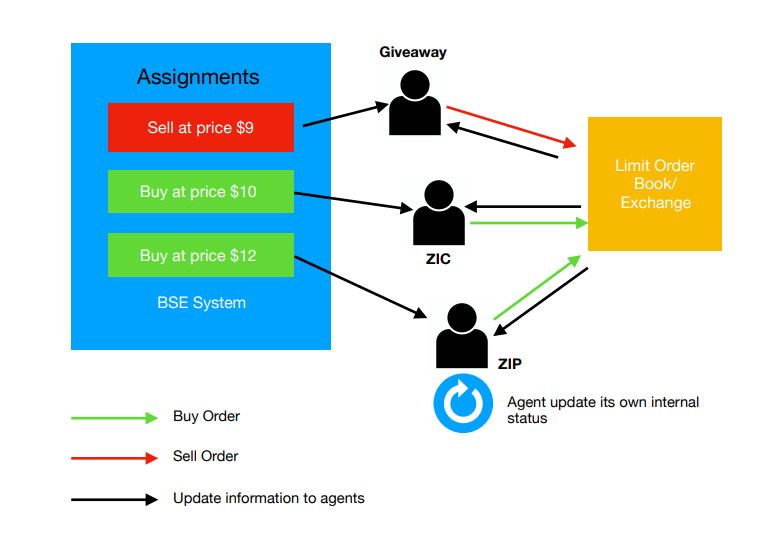
\includegraphics[ height=8cm]{BSE_figure}
\caption{McG's market model diagram} 
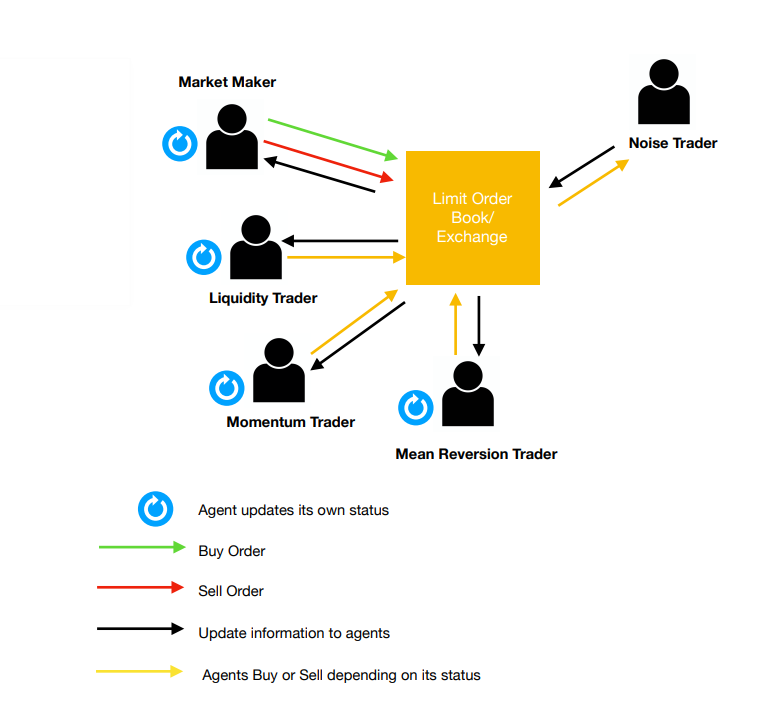
\includegraphics[width=12cm, height=10cm]{McGroarty_figure}
\end{figure} 
\FloatBarrier

In the new implementation which this project is trying to achieve is finding a way to integrate these two systems so that the McG agents will be able to mimic the real market environment for the agents such as ZIP, ZIC and AA implemented in the BSE. This implementation requires a few changes.

\begin{itemize}
    \item  \textbf{Quantity} : The current version of the BSE does not support orders with quantity more than 1. This has to be change because all of McGroarty et al. agents require their market to be able to receive orders with quantity more than 1. 
    \item  \textbf{Accepting more than one order per round}: In the current version, the BSE only accepts one order randomly from an agent in a action step. Agents such as the Market maker must be able to submit more than one order in every round. 
    \item \textbf{Deleting an order} : The current version of the BSE does not fully support an agent cancelling their order directly. This has to be implemented as a part of the system since McGroarty et al. agents are capable of cancelling an order.
\end{itemize} 

\section{Best Price in the BSE}
Some of McG's agents depend on the ``best price" of a side of the book in order to submit an order. However, unlike the real exchange market, the BSE does not always provide that, more specifically in the beginning of the trading day. This means that there must be some unavoidable modifications to the McG's agents condition regarding order submission. Instead of receiving the best price in each iteration from the LOB directly, the agents themselves will store their own best prices, both ask and bid. These values will be updated each time an order is processed and at the end of each action-step. 



\section{Time-step and real market dynamics}
The BSE time-step is easier to understand by giving an example. In a 300 BSE time-step, it is further divided into smaller steps which is equal to the total agents in the market. For example, if there are total of 14 agents in the market, the total number of time-steps in the 300 time period is $300 * 14 = 4200$. In these smaller time-step, an agent is chosen randomly to act in each time-step. 

In their paper, McG suggests that a new system to selecting agents will lead to a more realistic market. Unlike the BSE, the McG ensures that each agent has to act in every action-step. However, this is also dependent on a probability because in the real market, even if the price changes, not every high-frequency will be able to follow up and act on it. The probability is implemented based on this assumption. In addition, while BSE agents are required to submit an order if they are selected, the McG agents have two other options of submitting nothing or cancel their order(s). 

However, this leads to a slight problem. By implementing McG style of agent selection without probability of acting,the number of orders in the market will increase which leads to agents such as ZI-P not converging to the equilibrium correctly. This can be solved by introducing the probability of acting for each agent, much like the McG agents. A detailed investigation is presented in section 4.3. 

\section{Merging assignment based BSE system and McG ``best price" system}
The first change that must be made is that the BSE will give out order assignments to every agent except the McG agents. This will ensure that agents such as ZI-P, ZI-C or Sniper will perform correctly while running along the McG agents. Secondly, to solve the problem of the best price, one of the strategies from section 2.3 must be implemented. The McG agents will need to be adapt to include probability of acting because the selection of agents is now changed. 


\begin{figure}[!htbp]
\caption{BSE and McG merging market system diagram} 
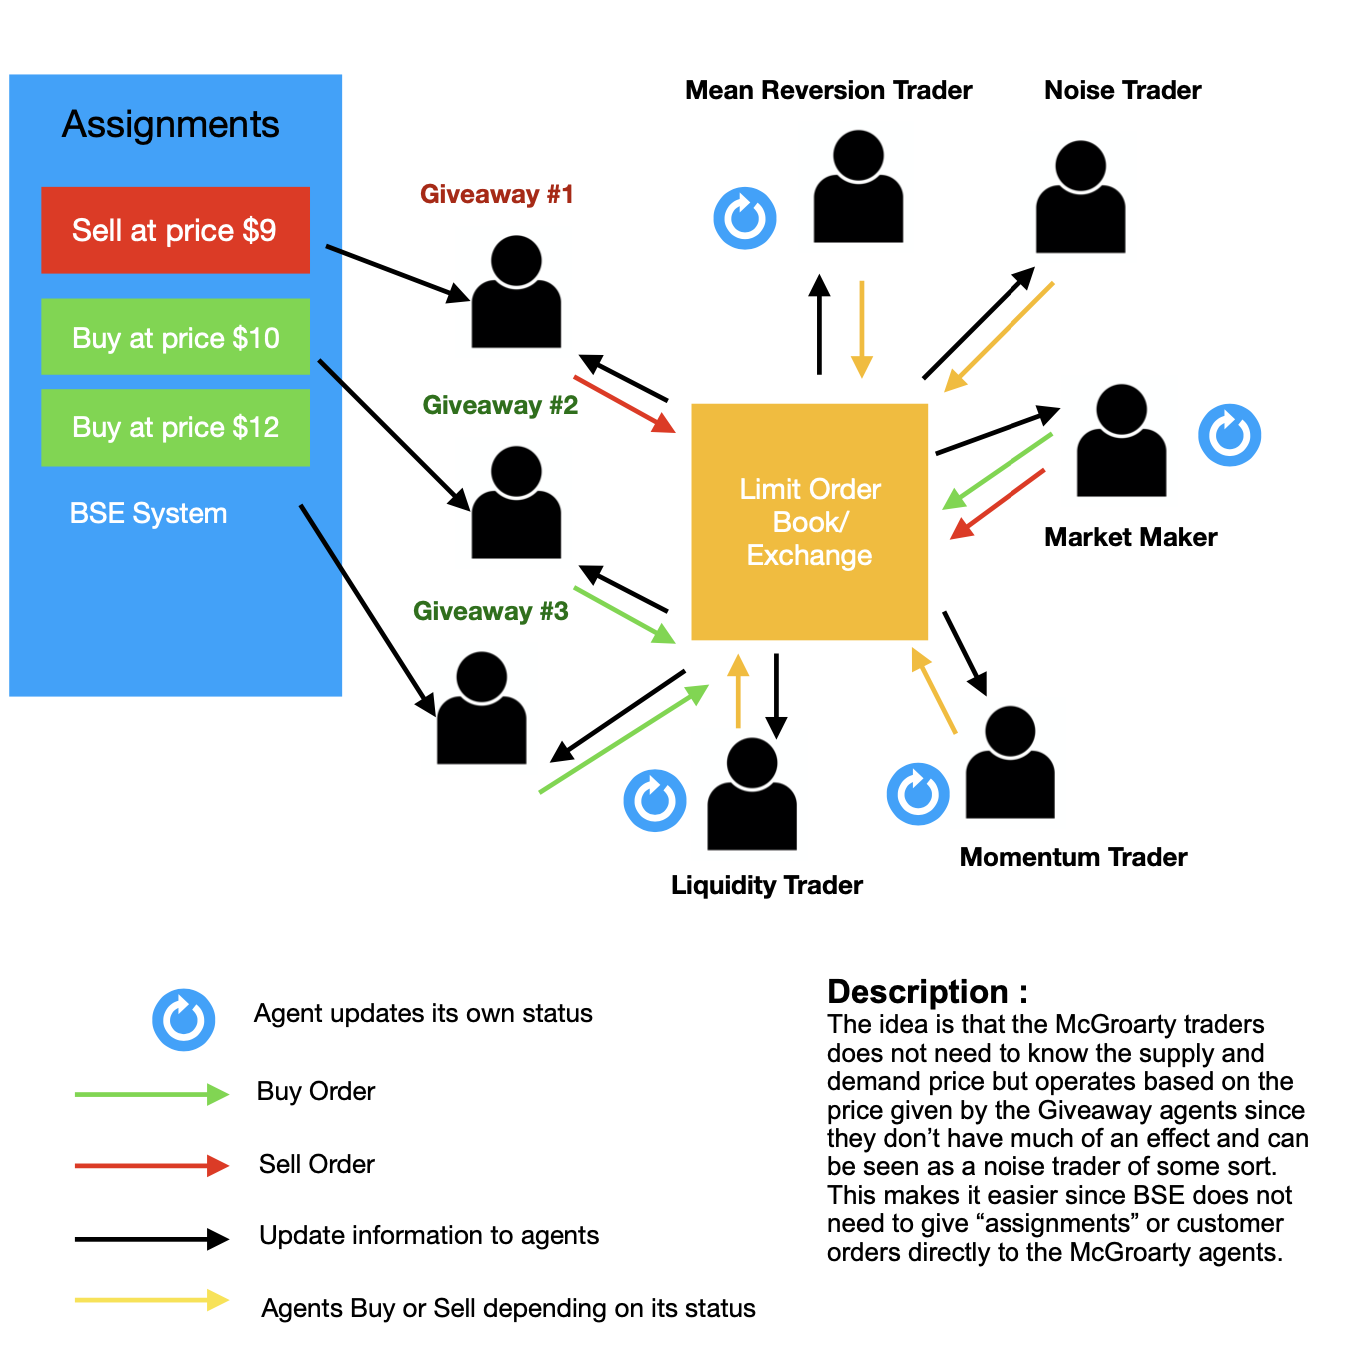
\includegraphics[width=16cm,height=16cm]{Dissertation/images/merge_bse_mcg.png}
\end{figure} 
\FloatBarrier

% \end{document} 